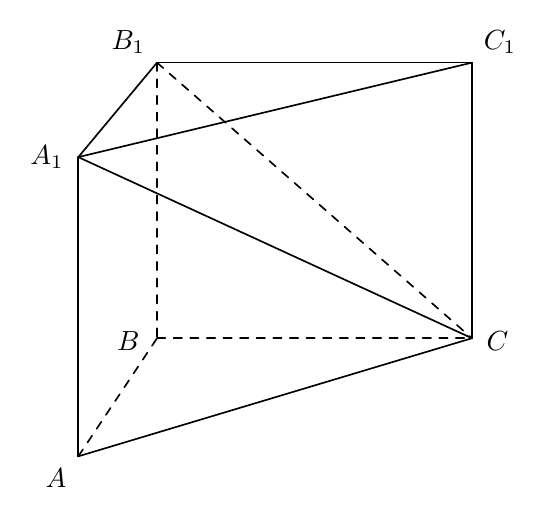
\begin{tikzpicture}[line width=.6pt, line join=round, line cap=round]
% 直三棱柱 ABC-A1B1C1  oblique sketch
\coordinate (B1) at (1.5,5.0);
\coordinate (C1) at (5.5,5.0);
\coordinate (A1) at (0.5,3.8);
\coordinate (B) at (1.5,1.5);
\coordinate (C) at (5.5,1.5);
\coordinate (A) at (0.5,0.0);
% visible solid edges
\draw (B1) -- (C1);
\draw (A1) -- (B1);
\draw (A1) -- (C1);
\draw (A1) -- (A);
\draw (C1) -- (C);
\draw (A) -- (C);
\draw (A1) -- (C);
% hidden dashed edges
\draw[dashed] (B1) -- (B);
\draw[dashed] (B) -- (C);
\draw[dashed] (A) -- (B);
\draw[dashed] (B1) -- (C);
% labels offset to avoid touching strokes
\node[font=\normalsize, inner sep=1pt, above left, xshift=-3pt, yshift=2pt] at (B1) {$B_{1}$};
\node[font=\normalsize, inner sep=1pt, above right, xshift=3pt, yshift=2pt] at (C1) {$C_{1}$};
\node[font=\normalsize, inner sep=1pt, left, xshift=-4pt] at (A1) {$A_{1}$};
\node[font=\normalsize, inner sep=1pt, left, xshift=-5pt, yshift=-1pt] at (B) {$B$};
\node[font=\normalsize, inner sep=1pt, right, xshift=4pt, yshift=-1pt] at (C) {$C$};
\node[font=\normalsize, inner sep=1pt, below left, xshift=-3pt, yshift=-3pt] at (A) {$A$};
\end{tikzpicture}
